\section{Improved parallel composition}\label{se-main}

The improved parallel composition algorithm extends the
conventional one by adding a pre-processing step, where some
places are removed from the components, as they are guaranteed
to be implicit in the result. To identify these places, one can
note that a place is required in the final composition only if
under some reachable marking it can be the only place that
disables some transition in its postset.

For simplicity, consider the parallel composition
$C=C_1\parallel C_2$, whose components synchronise on a single
signal $s$ which is an output of $C_1$ and an input of $C_2$.
Let $(M_1,M_2)$ be a reachable marking of $C$, where $M_1$ and
$M_2$ are some reachable markings of $C_1$ and $C_2$,
respectively. Furthermore, suppose that $M_1$ enables, say,
$s^+$ in $C_1$, where $s$ is an output. Now, if $M_2$ does not
enable $s^+$ in $C_2$, where $s$ is an input, then there is
computation interference. Therefore, if the FCI assumption
holds, $M_2$ has to enable $s^+$ in $C_2$, \ie whenever $s^+$
is enabled in $C_1$, it is also enabled in $C_2$. In other
words, the firing of $s^+$ in $C$ is fully controlled by $C_1$,
and so \emph{the constraints on firing of $s$ that are present
in $C_2$ can be ignored.} This means that the places in the
preset of an $s^+$-labelled transition in $C_2$ will be
implicit in the composition (subject to some technical
conditions formulated below), and so can be removed before the
composition is performed.

The above is true for the simple case of STGs with injective
labelling and no dummies. However, the general picture is more
complicated. In case of non-injective labelling, there can be
multiple transitions corresponding to the same input signal
transition, and the FCI assumption only guarantees the
enabledness of one of them. Hence, some `memory' (in the form
of places) is required to trace which of these transitions has
to be fired, which prohibits the removal of places from their
presets. Furthermore, if the STG contains dummies, removing
places from their postsets introduces some undesirable effects
explained later. These considerations lead to the following
conditions of applicability of the proposed optimisation.

\begin{proposition}\label{pr-main}
Let $C\DEF\parallel_{i\in I}C_{i}$ be a composition of STGs
that satisfies the FCI property and yields an
output-determinate STG, and, for each $i\in I$, $C_{i}'$ be the
STG obtained from $C_{i}$ by deleting all places $p$ such that:
\begin{enumerate}[1.]
\item each transition $t\in\post{p}$ is labelled with a
    signal, say $s$, and:
\begin{enumerate}[a)]
\item\label{only-inputs-in-postset} $s$ is an input;
\item\label{exists-matching-output} there is an STG $C_j$ for which $s$ is an output;
\item\label{injective-labelling} there are at most one
    $s^+$- and at most one $s^-$-la\-bel\-led
    transition in $C_i$;
\end{enumerate}
\item\label{no-dummies-in-preset} $\pre{p}$ does not
    contain dummy transitions.
\end{enumerate}
Then $C'\DEF\parallel_{i\in I}C_i'$ and $C$ have isomorphic
reachability graphs.
\end{proposition}
\begin{proof}
First of all, observe that $C'$ can be obtained from $C$ by
deleting some places. Hence, $\RG(C)$ is a subgraph of
$\RG(C')$, with the same initial state. Therefore it only
remains to show that there are no additional states or arcs in
the latter. For this, it is enough to show that for every state
$x$ of $\RG(C)$, the outgoing arcs of $x$ are the same in both
graphs. For the sake of contradiction, suppose there is a state
$x$ of $\RG(C)$ that has an outgoing arc $a$ that is in
$\RG(C')$ but not in $\RG(C)$.

The absence of $a$ in $\RG(C)$ means that some of the deleted
places $p$ was in $\pre{t}$ for some transition~$t$
corresponding to the arc $a$ in some of the component STGs
$C_i$, and the number of tokens in this place at state $x$ is
smaller than the weight of the arc $(p,t)$ in $C_i$ (*). Since
by condition~\ref{only-inputs-in-postset} $\post{p}$ can
contain only input transitions, $t$ must be labelled by
$s^\pm$, where $s$ is an input signal of $C_i$; \wlogg, we
assume that the label is $s^+$. By
condition~\ref{exists-matching-output} there is also a
component STG $C_j$ where $s$ is an output signal.

Let $\sigma$ be an execution of $C$ terminating at state $x$,
and $\nu$ be the trace corresponding to $\sigma$ (note that
such a $\sigma$ always exists as the reachability graphs
contain only reachable states). We proceed by showing that (i)
$\nu|_{C_j}s^+$ is a trace of $C_j$ and (ii) $\nu\, s^+$ is not
a trace of $C$; these would mean that there is a violation of
FCI in the original composition, leading to a contradiction.

(i) Since the arc $a$ is present in $\RG(C')$, the marking of
$C_j'$ corresponding to the global state $x$ enables some
$s^+$-labelled transition $t_j$ in it. Since $s$ is an output
in $C_j$, no places were removed from $\pre{t_j}$ when building
$C_j'$ due to condition~\ref{only-inputs-in-postset}, which
means that $t_j$ is also enabled by the marking of $C_j$
corresponding to the global state $x$, and so $\nu|_{C_j}s^+$
is a trace of $C_j$.

(ii) For the sake of contradiction, suppose $\nu\,s^+$ is a
trace of $C$. Due to the output-determinacy of $C$, the set of
outputs by which $\nu$ can be extended is uniquely determined,
and so $s^+$ must be enabled by $x$ (perhaps, after firing
several dummy transitions). By
condition~\ref{injective-labelling} there is only one
$s^+$-labelled transition in $C_i$ (\viz $t$), and so each
$s^+$-labelled transition in $C$ has $p$ in its preset with the
arc from $p$ to this transition having the same weight as the
arc $(p,t)$ in $C_i$. Consequently, each $s^+$-transition in
$C$ is blocked at state $x$ because by (*) the number of tokens
in $p$ is smaller than the weight of the corresponding arc.
Moreover, firing only dummy transitions cannot increase the
number of tokens in $p$ and thus enable an $s^+$-labelled
transition, as by condition~\ref{no-dummies-in-preset}
$\pre{p}$ contains no dummy transitions, a contradiction. Hence
$\nu\,s^+$ is not a trace of $C$.

As explained above, (i) and (ii) imply a violation of FCI and
so lead to a contradiction, which means that $\RG(C)$ and
$\RG(C')$ must be isomorphic.
\end{proof}

We now discuss the conditions of Prop.~\ref{pr-main} in more
detail. The conditions~\ref{only-inputs-in-postset}
and~\ref{exists-matching-output} are intrinsic to the proposed
method, and essentially state that due to the FCI assumption,
firing of an input signal in a component can be controlled from
the outside (\viz by the component controlling the
corresponding output --- whose existence is ensured
by~\ref{exists-matching-output}), and so the component itself
can get rid of the places controlling it.

The conditions~\ref{injective-labelling}
and~\ref{no-dummies-in-preset} are technical restrictions on
application of our method. If
condition~\ref{injective-labelling} is violated, there are
several transitions that have the same label, say $s^+$ (where
$s$ is an input) in the component. When the corresponding
output $s^+$ is produced by some other component, only one of
these transitions should fire to match it --- but to know which
one, the component needs to control their firing, and so the
places in their presets cannot be removed.

The necessity of condition~\ref{no-dummies-in-preset} is
illustrated by Fig.~\ref{fi-dummy-counterexample}. Intuitively,
the original STG on the left either receives $a^+$ followed by
$b^+$ without outputting anything, or receives $b^+$ and
produces $x^+$ in response. However, if the places in front of
$a^+$ and $b^+$ are removed (which would be possible without
condition~\ref{no-dummies-in-preset}), as shown on the right,
then it might produce the unexpected $x^+$ after the trace
$a^+\,b^+$. Intuitively, in the initial STG firing of $a^+$
acts as an evidence that the dummy transition in the right
branch has fired, while in the modified one the postset of this
dummy transition has been removed, and so it is not possible
anymore to guarantee that it has fired when $a^+$ fires.

\begin{figure}[!tb]
    \centering
    {}%
    \hfill%
    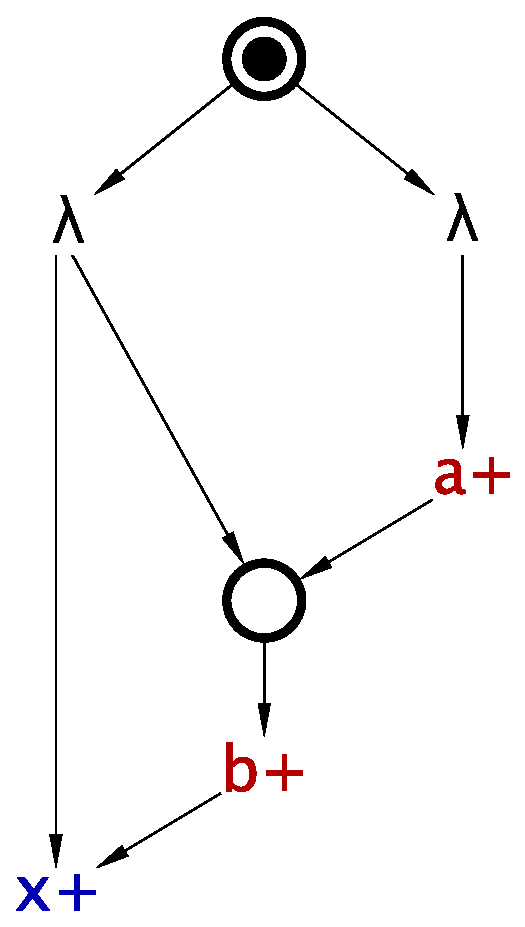
\includegraphics[scale=0.3]{EXPERIMENTS/stg/dummy_counterexample}%
    \hfill%
    \raisebox{5.9em}[5.9em][0em]{\Large$\Rightarrow$}
    \hfill%
    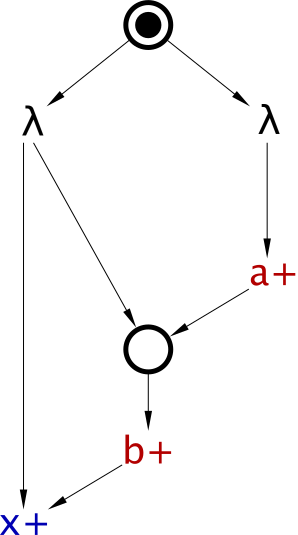
\includegraphics[scale=0.3]{EXPERIMENTS/stg/dummy_counterexample_removed}%
    \hfill%
    {}
    \caption{\label{fi-dummy-counterexample}
        Example of an STG where removal of places in the postset of dummy transitions results in a wrong behaviour.
    }
\end{figure}


In practice, when performing the parallel composition, one
would like as few implicit places as possible in the result,
and so it would be desirable to weaken the conditions in
Prop.~\ref{pr-main}, so that as many places as possible are
removed. As the conditions~\ref{only-inputs-in-postset}
and~\ref{exists-matching-output} are intrinsic, it is unlikely
that they can be relaxed. However, the technical
conditions~\ref{injective-labelling}
and~\ref{no-dummies-in-preset} can be dealt with --- by
ensuring that the components always satisfy them. Indeed, as
mentioned in Sect.~\ref{sec_pn_basic}, for output-determinate
STGs the language is the semantics, and so one often can remove
dummy transitions and enforce injective labelling without
changing the language, \eg using the \petrify
tool~\cite{ckkly97}; this will ensure that
conditions~\ref{injective-labelling}
and~\ref{no-dummies-in-preset} hold. An example of such a
transformation for the \balsa standard component Call is shown
in Fig.~\ref{fi-enforce-inj}. This operation is performed on
(small) components rather than the (large) composition, and so
is usually cheap. Moreover, in some applications, in particular
circuit re-synthesis, the components are taken from a fixed
library of component types, and so the transformation can be
performed only once for each component type, and subsequently
incur no runtime penalty at all.

\begin{figure}[!tb]
    \centering
    {}%
    \hfill%
    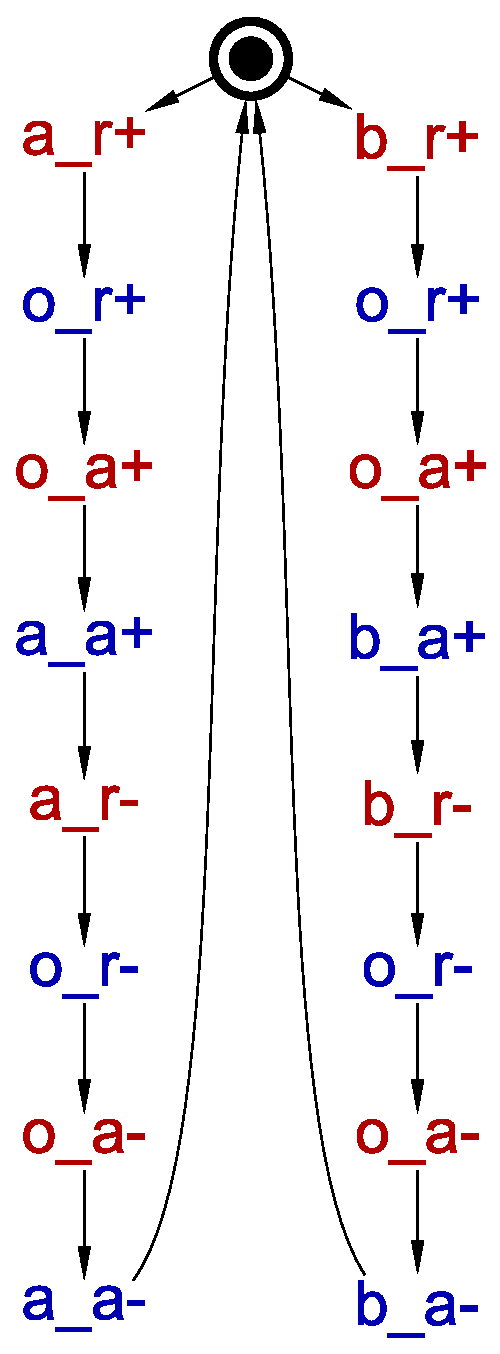
\includegraphics[scale=0.3]{EXPERIMENTS/stg/mix_full}%
    \hfill%
    \raisebox{8.9em}[8.9em][0em]{\Large$\Rightarrow$}
    \hfill%
    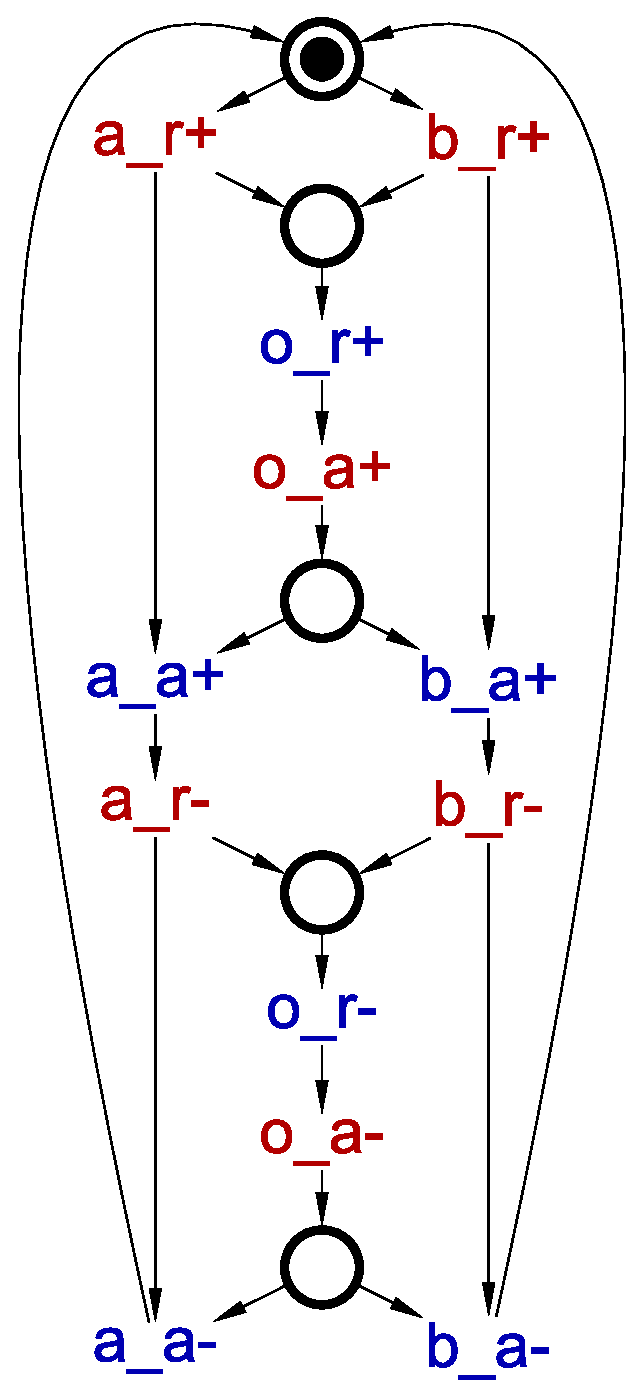
\includegraphics[scale=0.3]{EXPERIMENTS/stg/mix_full_inj}%
    \hfill%
    {}
    \caption{\label{fi-enforce-inj}
        Example of enforcing injective labelling in an STG.
    }
\end{figure}
